
\documentclass[10pt]{report}

\usepackage{url}
\usepackage{tabularx}
\usepackage{graphicx}
%\usepackage[boxed,linesnumbered,ruled,vlined]{algorithm2e}
%\usepackage{amssymb,amsmath,amsthm,amssymb}
\usepackage{multirow}
\usepackage{caption}
\usepackage{subcaption}
\usepackage{ctable}
\usepackage{balance}
\usepackage{listings}
%\usepackage{hyperref}


\begin{document}
%
% paper title
% can use linebreaks \\ within to get better formatting as desired
%\title{Topology-Aware Load Balancing for Parallel Applications on Multi-Core Systems}
%\title{Livrable 1.1.2\\}
\title{AGIOS User Guide}


\author{
Francieli Zanon Boito\\Universidade Federal do Rio Grande do Sul (UFRGS)\\Porto Alegre, Brazil\\\\(Past)\\Laboratoire d'Informatique de Grenoble (LIG) - INRIA\\Universit\'{e} Grenoble Alpes\\Grenoble, France}

\date{August 2015}

% make the title area
\maketitle

\tableofcontents


\chapter{Introduction}

This document describes \emph{AGIOS}\footnote{The tool's name - AGIOS - comes from ``Application-Guided I/O Scheduler'' and is Greek for ``holy''.}. 

\textbf{(If you already know AGIOS and/or are in a hurry, you can skip this introduction and some chapters. Please read this document in this order: Chapter~\ref{chapter:starting}, \ref{chapter:serra}, \ref{chapter:configfile}, and then Chapter~\ref{chapter:citing}.)}

The main objectives for AGIOS' development were to make it generic, non-invasive, easy to use, and to offer multiple choices on scheduling algorithms.

We wanted to develop a tool that could be used by \emph{any I/O service that treats requests at a file level}, such as a local file system or intermediate nodes in an I/O forwarding scheme. For this reason, AGIOS has a library implementation suitable for inclusion on most of today's parallel file systems' servers. On the other hand, AGIOS also offers a kernel module implementation that can be used, for instance, at the virtual file system layer. The I/O services that use AGIOS are called its ``users''. Our AGIOS implementation is deeply inspired by the aIOLi framework\footnote{\url{http://aioli.imag.fr/}}.

\begin{figure}[!h]
\centering
\begin{subfigure}{0.4\textwidth}
\centering
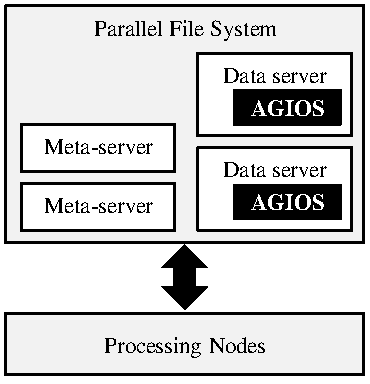
\includegraphics[width=\textwidth]{images/agios_usage_example_1.pdf}
\caption{in a parallel file system's data servers}
\label{fig:agios_usage_example_1}
\end{subfigure}
\hspace{1cm}
\begin{subfigure}{0.4\textwidth}
\centering
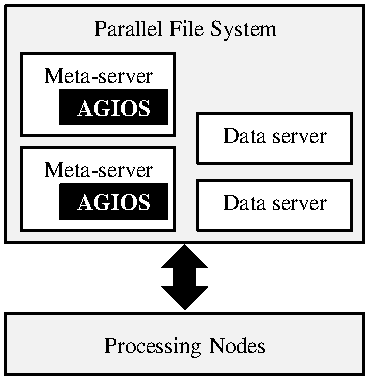
\includegraphics[width=\textwidth]{images/agios_usage_example_2.pdf}
\caption{in a parallel file system's metadata servers}
\end{subfigure}
%\vspace{1cm}
\begin{subfigure}{0.4\textwidth}
\centering
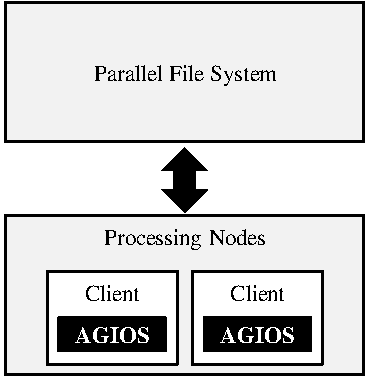
\includegraphics[width=\textwidth]{images/agios_usage_example_3.pdf}
\caption{in the processing nodes (either local VFS or PFS client)}
\end{subfigure}
\hspace{1cm}
\begin{subfigure}{0.4\textwidth}
\centering
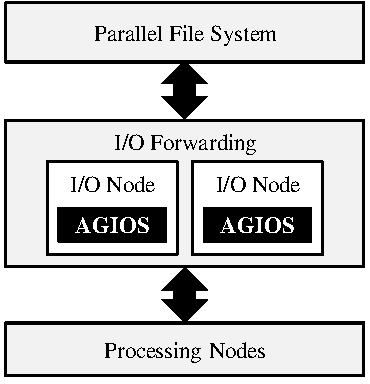
\includegraphics[width=\textwidth]{images/agios_usage_example_4.pdf}
\caption{in the intermediate nodes from an I/O forwarding scheme}
\end{subfigure}
\caption{Four examples of use for AGIOS.} \label{fig:agios_usage_examples}
\end{figure}

Figure~\ref{fig:agios_usage_examples} presents four non exhaustive examples of use for AGIOS. All of the four presented placement options are I/O services that treat requests at a file level, and are places where it makes sense to use I/O scheduling. These placement options are not exclusive, in the sense that we could have all of them happening at the same time. In order to avoid creating a bottleneck, AGIOS instances (on different PFS servers, or at different levels of the I/O stack) are independent and do not make global decisions. 

AGIOS exports a simple interface composed of four steps:

\begin{itemize}

  \item \textbf{Initialization:} The user calls \emph{agios\_init} in order to initialize the AGIOS infrastructure. At this moment, the user must provide a callback function used to process a single request. If a function capable of processing a list of requests at once is available, the user should also provide it.

  \item \textbf{A new request arrives:} The user calls \emph{agios\_add\_request} to transmit the request to the scheduler.

  \item \textbf{Requests are ready to be processed:} The scheduler passes the requests back to its user through the provided callback function. Therefore, the task of processing requests is left to the I/O services using the library.
    This keeps AGIOS' interface simple and generic.

  \item \textbf{Finalization:} The user calls \emph{agios\_exit} for cleaning up the tool's infrastructure.

\end{itemize}

\begin{figure}[h]
\centering
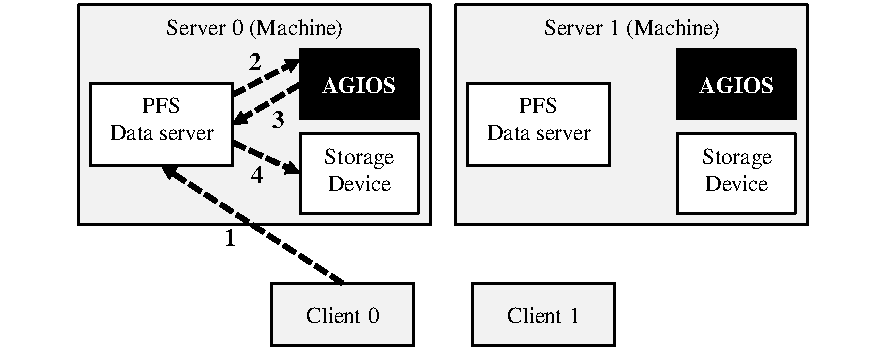
\includegraphics[width=\columnwidth]{images/agios_interface.pdf}
\caption{A request's path to a PFS server with AGIOS.} \label{fig:agios_interface}
\end{figure}

Additional calls are provided to generate access statistics files and to reset statistics.
An illustration of this interface is provided in Figure~\ref{fig:agios_interface}, that shows a situation where AGIOS is used by a parallel file system's data servers (scenario illustrated at Figure~\ref{fig:agios_usage_example_1}). In step \textbf{1}, a server receives requests. It transmits the requests to the scheduler in step \textbf{2}. After applying a scheduling algorithm, AGIOS will give requests that are ready to be processed back to the server in step \textbf{3}. In step \textbf{4}, the server will process the requests. This whole process could also be happening in the other server, without	affecting the first one. 

Virtual requests obtained by aggregating single requests will be served together if the library user (the server) provided a callback for this functionality.
Otherwise, the
original requests selected for aggregation will be served
sequentially. However, even when it is not possible to effectively
aggregate requests into larger ones, performance can still benefit
from the execution of contiguous requests served in offset order instead
of the original random order. Moreover, other levels of the I/O stack might aggregate these requests.
% show that it does not really make a difference (with an experiment)

I/O scheduling is mainly meant for
multi-application scenarios, aiming
at avoiding the ill effects of interference in applications'
performance. Additionally, different processing nodes can also interfere with each other even when executing the same application.
Users such as parallel file systems' servers are often unable to determine from which application or process requests are coming, since this information is lost through the I/O stack.
For this reason, the scheduler works in the context of files instead of
applications. 
Moreover, the scheduler is able to provide performance improvements even on single-application scenarios.

The rest of this report provides the required knowledge to use AGIOS. We assume the reader is familiar with the programming language C and has at least basic notions about the \emph{Pthreads} API. The tool has two implementations: an user-level library and a kernel module. Nonetheless, since the kernel module implementation is still experimental, we only cover the library version in this document.  The next chapter discusses its installation and interface to users. Chapter~\ref{chapter:algorithms} presents the five available scheduling algorithms, and Chapter~\ref{chapter:trace} discusses trace files generation and the Prediction Module. How information about storage devices - obtained from another tool - should be provided to AGIOS is the subject of Chapter~\ref{chapter:serra}. Chapter~\ref{chapter:configfile} presents the configuration file format and the meaning of its parameters. Finally, Chapter~\ref{chapter:citing} provides publication and contact information. 


\chapter{Getting Started} \label{chapter:starting}

AGIOS' code can be retrieved from \url{https://bitbucket.org/francielizanon/agios/wiki/AGIOS-1.0.tgz}. You will need to download it, compile and install.

\begin{lstlisting}[language=bash]
$ tar xzf AGIOS-1.0.tgz
$ cd AGIOS-1.0/
$ make clean
$ make library
$ make install
\end{lstlisting}

The commands above will install the library in \emph{/usr/lib/} and copy its header - \emph{agios.h} -  to \emph{/usr/include}. It requires that \emph{Libconfig} is installed, you can get it from \url{http://www.hyperrealm.com/libconfig/}. 

AGIOS can then be used in your I/O service's code through:

\begin{lstlisting}[language=C]
#include <agios.h>
\end{lstlisting}

\section{Initialization}

As previously discussed, AGIOS' interface is composed of two main steps: requests are added to the scheduler, and a callback is used to notify the user it is time to process requests. 

The first thing is to initialize the library. A \emph{struct client} must be filled before calling \emph{agios\_init}:

\begin{lstlisting}[language=C]
struct client {
	void (*process_request)(int i);
	void (*process_requests)(int *i, int reqnb);
	short int sync; 
};
\end{lstlisting}

The user must provide at least the \emph{process\_request} callback, used by the scheduler to process a request. As previously discussed, a callback to process multiple requests at once can also be provided: \emph{process\_requests}. 

Notice that requests are identified between user and scheduler through an integer value. This value is managed by the user and provided to the scheduler in the \emph{agios\_add\_request} call.

\begin{lstlisting}[language=C]
int main()
{
	struct client clnt;
	char *config_filename = "/tmp/agios.conf";

	clnt.process_request = my_process_request_function;
	clnt.process_requests = NULL;

	agios_init(&clnt, config_filename);

	...
}
\end{lstlisting}

The above code initializes the library, passing a callback function to process a request, but not to process multiple requests at once (in this case it should be set to NULL). 

\begin{lstlisting}[language=C]
int agios_init(struct client *clnt, char *config_file);
\end{lstlisting}

Notice that the \emph{agios\_init} call also requires the name for a configuration file. Chapter~\ref{chapter:configfile} discusses the configuration file.

The initialization function will return $0$ in case of success and something else in case of errors.

\begin{lstlisting}[language=C]
	agios_init(&clnt, config_filename);
	if(clnt.sync)
		...
\end{lstlisting}

During initialization, AGIOS will decide which I/O scheduling algorithm to use. Some of them require synchronous scheduling, i.e. one request must be processed at a time, and the scheduler will only choose more requests after the previous were processed. The responsibility of making this synchronization is left to users in order to keep the library as generic as possible. An example of how this can be done will be provided in the next section.

\section{Scheduling requests}

When requests arrive to the user, they must be provided to AGIOS through the \emph{agios\_add\_request} call.

\begin{lstlisting}[language=C]
int agios_add_request(char *file_id, int type, 
		      long long offset,long len, 
		      int data, struct client *clnt);
\end{lstlisting}

The first parameter - \emph{file\_id} - is an identifier of the file this request is for. It is a good idea not to use simply a file handler but an unique identifier that will always be the same to each file (such as the file's name). 

The request's \emph{type} must be \emph{RT\_READ} or \emph{RT\_WRITE}, according to the operation being performed.

\emph{Offset} and \emph{len} give the file position where to start the operation and its size, respectively.

\emph{Data} is the integer value that identifies the request to the user. It will be provided by the scheduler when processing this request. For instance, if requests are added to an array in the user, a good choice would be to provide the request's index in this parameter.

The \emph{struct client} parameter is the same initialized and provided to \emph{agios\_init}.

Once requests are ready to be processed, the scheduler will call the \emph{process\_request} callback previously discussed, giving back the provided \emph{data} parameter of the requests. This function should return as soon as possible so the scheduler can continue to select requests to be processed, unless the field \emph{sync} from the struct client was set to $1$ during the initialization phase. In this case, the library's user must ensure the synchronization. The code below provides a simplified example of how this can be done with \emph{pthread} condition variables.

\begin{lstlisting}[language=C, breaklines=true]
#include <pthread.h>
#include <agios.h>

#define CONFIG_FILE "/tmp/agios.conf"

short int agios_can_continue=0;
pthread_cond_t req_processed_cond = 
				PTHREAD_COND_INITIALIZER;
pthread_mutex_t req_processed_mutex = 
			       PTHREAD_MUTEX_INITIALIZER;
struct client clnt;

void receiver_thread()
{
   int index, type;
   char *file_id;
   long long offset;
   long len;

   do {
      index = receive_request_from_client
			(&file_id, &type, &offset, &len);
      agios_add_request
	       (file_id, type, offset, len, data, &clnt);
   } while(!end_of_execution());
}

void io_thread()
{
   int index;

   do {
      index = wait_for_ready_requests();
      process_ready_request(index);

      /*notify that AGIOS can proceed*/
      if(clnt.sync)
      {
         pthread_mutex_lock(&req_processed_mutex);
	 agios_can_continue=1;
	 pthread_cond_signal(&req_processed_cond);
	 pthread_mutex_unlock(&req_processed_mutex);			
      }
   } while(!end_of_execution());
}

void my_process_request_callback(int i)
{
   notify_io_thread_about_ready_request(i);

   /* wait until it was processed before AGIOS 
    * can schedule more requests */
   if(clnt.sync)
   {
      pthread_mutex_lock(&req_processed_mutex);
      while(!agios_can_continue)
         pthread_cond_wait
	     (&req_processed_cond, &req_processed_mutex);
      agios_can_continue=0;
      pthread_mutex_unlock(&req_processed_mutex);
   }
}

int main()
{
   /* initialize AGIOS*/
   clnt.process_request = my_process_request_callback;
   clnt.process_requests = NULL;
   it(agios_init(&clnt, CONFIG_FILE) != 0)
   {
	exit_on_error();
   }

   /*initialize threads*/
   start_receiver_thread();
   start_io_thread();

   ...
}

\end{lstlisting}

In this example, the I/O service has two main threads: the receiver thread, responsible for receiving requests from the I/O service's clients, and the I/O thread, which treats the requests (performs I/O). The receiver thread gives incoming requests to AGIOS, which calls \emph{my\_process\_request\_callback()} when they are ready to be processed. This callback will notify the I/O thread, that will actually process requests. A \emph{pthread} condition variable (associated with a mutex) ensures the synchronous behavior when required by AGIOS.

\section{Generating scheduling statistics}

During execution, the AGIOS' user can ask the library to generate statistics files through the \emph{agios\_print\_stats\_file} call. This call may take a long time if called too soon after the library's initialization, before the Prediction Module is initialized (because it will have to wait for it).

\begin{lstlisting}[language=C]
void agios_print_stats_file(char *filename);
\end{lstlisting}

Statistics can be reset by calling \emph{agios\_reset\_stats}. If trace files are being generated, this call will result in closing the actual trace file and starting a new one. If the Prediction Module is reading from trace files, it will take the just-closed trace file and consider it in its decisions. More detail on trace files and the Prediction Module will be presented in Chapter~\ref{chapter:trace}.

\begin{lstlisting}[language=C]
void agios_reset_stats(void);
\end{lstlisting}

\section{Ending the execution}

When finishing the I/O service execution, the \emph{agios\_exit} function must be called.

\begin{lstlisting}[language=C]
void agios_exit(void);
\end{lstlisting}


\chapter{I/O Scheduling Algorithms} \label{chapter:algorithms}

This chapter presents the five scheduling algorithms available with AGIOS: aIOLi, SJF, TO, and TO-agg. These algorithms were selected for their variety, in order to represent different situations and complement each other's characteristics.

\section{aIOLi} \label{sec:agios_aioli}

We have adapted the \emph{aIOLi} scheduling algorithm from Lebre et al. A full explanation and discussion about this algorithm's characteristics can be found in the paper that describes it\footnote{A. Lebre, Y. Denneulin, G. Huard, and P. Sowa, “I/o scheduling service for multi-application clusters,” in Proceedings of IEEE Cluster 2006, conference on cluster computing, sep 2006.}, but we can summarize it as follows:

\begin{itemize}

  \item Whenever new requests arrive to the scheduler, they are inserted in
    the appropriate queue according to the file to be accessed. There are two
    queues for each file: one for reads, and another for writes.

  \item New requests receive an initial quantum of 0 bytes. 

  \item Each queue is traversed in offset order and aggregations of
    contiguous requests are made. When an aggregation is performed, a
    \emph{virtual request} is created, and this request will have a quantum
    that is the sum of its parts' quanta.

  \item All quanta (including the virtual requests' ones) are increased by a value that depends on its queue's past quanta usage.

  \item In order to choose a request to be served, the algorithm uses an
    offset order inside each queue and a FCFS criterion between
    different queues. Additionally, to be selected, the request's
    quantum must be large enough to allow its whole execution (it needs to match the request's size). 

  \item The scheduler may decide to wait before processing some requests if a) a shift phenomenon is suspected or b) better aggregations were recently achieved for this queue.

  \item After processing a request, if there is quantum left, other contiguous request from the same queue can be processed - given that they fit the remaining quantum. After stopping for a queue, its quanta usage ratio is updated.
This scheduling algorithm works synchronously, in the sense that it waits until a virtual request is processed before selecting other ones.
\end{itemize}

The implementation uses a hash table indexed by file identifier for accessing the requests queues. 
At a given moment, the cost of including a new request to a queue can be represented as the sum of the required time to find the right queue plus the time to find its place inside the queue (sorted by offset order).  This cost is expected to be $O( (M / S_{hash}) + N_{queue} )$, where M is the number of files being concurrently accessed, $S_{hash}$ is the number of entries in the hash table, and $N_{queue}$ is the number of requests in the largest queue. Selecting a request for processing, on the other hand, involves going through all queues: $O( 2 \times M )$

\section{MLF}

Under a workload where several files are being accessed at the same time, the cost of aIOLi's selection may become a significant part of requests' lifetime in the server. This happens due to the synchronous approach where the algorithm waits until the previous request was served before selecting a new one. In order to have a scheduler capable of providing more throughput, we developed a variation of aIOLi that we called \emph{MLF}. 
%We have chosen this name because our version is closer to the traditional MLF task scheduling algorithm than aIOLi.

To reduce the algorithm's overhead, we removed the synchronization between user and library after processing requests. Therefore, the new algorithm works repeatedly, possibly overflowing its user with requests. 
%
Despite its possibly high scheduling overhead, one advantage of the synchronous approach is that having some time before the next algorithm's step gives chance for new requests to arrive and more aggregations to be performed. Therefore, it is possible that this new algorithm will not be able to perform as many aggregations as aIOLi. 

Other difference between MLF and aIOLi is that MLF does not respect a FCFS order between the different queues. Therefore, not all queues need to be considered before selecting a request, improving the algorithm's throughput.
MLF's cost for including new requests is the same as aIOLi's, but its cost for selection is $O(1)$.

\section{SJF} \label{agios_sjf}

We have also developed for our study a variation of the \emph{Shortest Job First (SJF)} scheduling algorithm that performs requests aggregation. Its implementation also uses two queues per file and considers requests from each queue in offset order. The selection of the next request is done by going through the queues and selecting requests from the smallest one (considering each queue's total size, i.e. the sum of all its requests' sizes).
%
Therefore, the cost for including a new request and for selection are the same as aIOLi's. However, as MLF, our SJF variation does not work synchronously.

\section{TO and TO-agg}

\emph{TO} is a timeorder algorithm. It has a single queue, from where requests are extracted for processing in arrival time order (FCFS). Both the costs of including and selecting requests are, therefore, constant. 
%We have included TO in our analysis to cover situations where no scheduling algorithm is able to improve performance. 

We have also included a timeorder variation that performs aggregations: \emph{TO-agg.} Since there is a single queue for requests, aggregating a request possibly requires going through the whole queue looking for a contiguous one. Therefore, this algorithm's cost for including requests is $O( N )$, where N is the number of requests currently on the scheduler. The time for selection is still constant. 



\chapter{Trace Files and the Prediction Module} \label{chapter:trace}

We have decided to use trace files to obtain information from applications because we wanted to keep AGIOS generic and easy to use. Most methods to obtain such information include changes in I/O libraries, compilers or applications, which would compromise the portability of our tool. The trace file is generated by the scheduler itself and stored on its local storage device, without modifications to the application or to the file system.

\begin{figure}[!b]
\centering
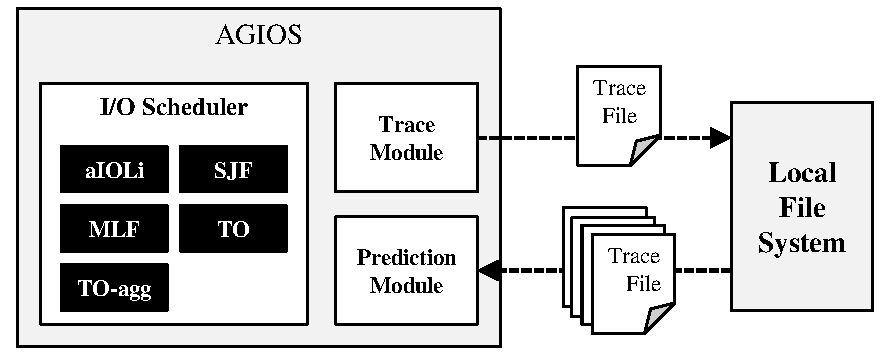
\includegraphics[width=\columnwidth]{images/agios_architecture.pdf}
\caption{AGIOS' modules and trace generation.}
\label{fig:agios_architecture}
\end{figure}

Figure~\ref{fig:agios_architecture} presents AGIOS' modules. 
Trace generation is activated by a configuration parameter, and can be used with any of the provided scheduling algorithms. The \emph{Prediction Module} is responsible for obtaining information from traces and providing them to scheduling algorithms.

The Prediction Module is initialized by the scheduler in the beginning of its execution if trace files are present. A prediction thread then reads the traces and generates a set of queues identical to the ones used during execution, except that these contain ``predicted'' future requests. This initialization can also be triggered during execution, providing the ability to generate a trace file during some initial period of the execution and then start the Prediction Module if we expect the traced access pattern to happen again in the future. This would be done through the \emph{agios\_reset\_stats} call, discussed in Chapter~\ref{chapter:starting}.

\section{Trace generation}

In the trace file, a ``new request'' entry stores the file identifier, offset, size, and timestamp of the request - the number of nanoseconds elapsed since the current trace's first request arrival, or $0$ in the case of the first request. 

Since writing information about requests to a local file could affect the scheduler's results, the Trace Module keeps a buffer. A large trace buffer minimizes the number of I/O operations to the trace file. On the other hand, a buffer that is too large could affect the whole I/O service's performance by increasing its memory footprint.

Different traces generated by executing the same application may present some variation between the arrival times of the same request. In order to obtain more realistic arrival time estimations, several trace files can be combined. Therefore, while reading predicted requests from trace files, the Prediction Module checks if they already exist in its queues. This comparison is done by file identifier, offset, size, and arrival times relative to the first request to the file. Requests are the same only if their arrival times difference is within a tolerance, provided from configuration parameters.

\section{Predicted aggregations}

From a set of predicted future requests, the Prediction Module can predict aggregations that will be possible during execution and provide this information to scheduling algorithms. These predictions require an $\alpha$ factor which represents the ability to overlap waiting times with processing requests from other queues. It is estimated at initialization time, and can be updated during execution time based on the real ability observed at the scheduler.

When an actual request arrives, the scheduler looks for predicted requests to the same file with the same offset, size and with a relative timestamp (relative to the first request to this file) within acceptable bounds. These ``acceptable bounds'' are defined by an acceptable error parameter, the same used while reading traces to decide if predicted requests are the same. If the scheduler finds such a request, the two versions (predicted and actual) are linked and the predictions concerning this request will be considered during scheduling. 

When a virtual request is selected to be served, the scheduler asks the
Prediction Module if it should be done now, or if it should wait
for some period. In order to make this decision, the Prediction Module
analyzes the aggregation predicted for the requests' traced versions. If the aggregation is not as big as the predicted one, the scheduler must wait. In order to avoid starvation, the wait will happen only once for each virtual request. 

This process, available only for I/O scheduling algorithms that have waiting times (aIOLi and MLF), is illustrated in Fig.~\ref{fig:scheduling_traces}. 
In the instant $t_1$, the scheduler needs to decide if it dispatches
    the three highlighted incoming requests for execution or if it waits for
    longer. With information from the trace, the scheduler knows that a bigger aggregation is possible for these requests.

\begin{figure}[!h]
  \centering
  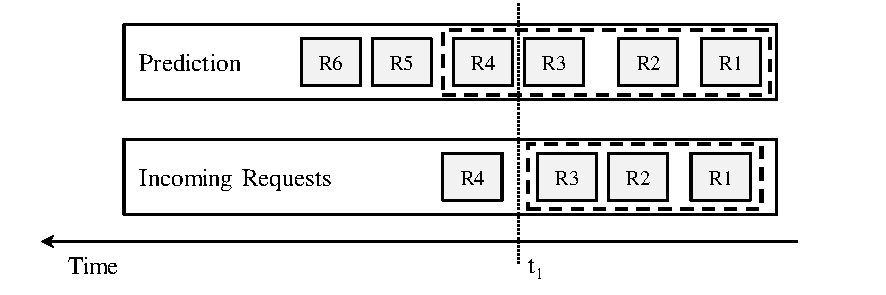
\includegraphics[width=\columnwidth]{images/app_sched.pdf}
  \caption{Scheduling with predicted future requests.}
  \label{fig:scheduling_traces}
\end{figure}

After processing actual requests, predicted versions will not be discarded. Therefore, repeating access patterns (or repeated executions of the same application) can benefit several times from the same predictions. Traces can be reused for applications' executions with different parameters as long as they do not change what file portions are accessed from each server.

\section{Access pattern detection}

Another functionality of the Prediction Module is access pattern detection. Through a decision tree (generated with machine learning techniques), it classifies applications' accesses in contiguous or non-contiguous and small or large. This decision is made from two metrics calculated to each file with predicted accesses. The general access pattern is considered to be the access pattern for the majority of the files.

The process of reading multiple trace files and combining them to generate predictions can be very time consuming. It is possible to enable the generation of simplified trace files by the Prediction Module. These files are generated after reading regular trace files and each one of them has the calculated metrics to a file with predicted requests. In future executions of AGIOS, it is possible to provide only these files (instead of the regular trace files). They will provide enough information to access pattern detection and scheduling algorithm selection, but not for predicting request aggregations.

\section{Scheduling algorithm selection}

The Prediction Module is also capable of selecting automatically the best fit in scheduling algorithm depending on the situation. This is also done through a decision tree, using the detected general access pattern and information about the storage device. For now, this selection is only available at initialization time, using information from traces.

Information about the storage device is obtained through .h files generated by SeRRa. This will be further discussed in the next chapter.

Both the access pattern detection and scheduling algorithm selection were designed for AGIOS' use by a parallel file system's data servers. For other situations, results should make no sense, so please avoid using these functionalities.



\chapter{Providing Information about the Storage Device with SeRRa} \label{chapter:serra}

As previously discussed, the Prediction Module requires information about the user's storage device to perform scheduling algorithm selection. Additionally, other parts of the library implementation also use this information. This information is provided to AGIOS through two a file generated by SeRRa. The tool and information on how to use it can be obtained at \url{http://serratool.bitbucket.org/}.

The file name (with its path) must be provided to AGIOS through its configuration file. The next chapter will give more details about the configuration file.

\begin{lstlisting}[language=bash]
2
8	64
566.8405	6784.471
238.2483	1173.456
145.6056	1018.143
187.2437	-201.8793
64	128
571.2364	-740.0433
234.6933	41.99119
218.3765	-6295.179
113.1743	2235.442
\end{lstlisting}

We show above an example of the file generated by SeRRa. This file gives estimated access times in the form of linear functions. The first line gives the number of considered intervals, and then intervals are described one after the other, in request size order. Each interval takes $5$ lines, where the first one gives the interval information. In this example, we have two intervals: [$8$KB, $64$KB] and [$64$KB, $128$KB]. The following $4$ lines define the access times functions for different access patterns in the following order: sequential write, random write, sequential read, and random read. In the example, the time to perform sequential write in the profiled storage device is given by \\
$time(request\_size) = 566.8405 \times request\_size + 6784.471 nanoseconds$.

If the library needs to estimate a request size which is not included in the described intervals, it will use the function provided for the last interval of this file. However, to have more accurate results, the following guidelines should be taken into consideration when generating the file with SeRRa:

\begin{itemize}
\item Describe intervals to SeRRa comprising at least requests from $4$KB to $4$MB. We suggest separating these values into two intervals, breaking at $64$KB. In our experience with multiple storage devices, this leads to the best results.
\item If you can afford the profiling time, use as many benchmark repetitions as possible (this is a parameter provided to SeRRa, see its documentation for more detail).
\item If you are using AGIOS on a Grid'5000 cluster, take a look at our page since we provide files obtained at some clusters.
\end{itemize}

The access time estimations are used by the aIOLi scheduling algorithm (to quantum assignment) and by the Prediction Module (to maintain the $\alpha$ factor and test against predicted aggregations). They are also used to the mechanism which automatically selects the best scheduling algorithm to obtain the sequential to random throughput ratio of the storage device. If you are using AGIOS without predicted request aggregations and with another scheduling algorithm (statically, without automatic scheduling algorithm selection), you can provide any values (the example file that comes within the library package is OK).



\chapter{The Configuration File} \label{chapter:configfile}

This chapter presents AGIOS' configuration file. As discussed in Chapter~\ref{chapter:starting}, a configuration file name (with path) must be provided in the \emph{agios\_init} call. The first thing in initialization phase is to read this file. If it is not present and complete, unexpected library behaviors may result.

AGIOS' configuration file is parsed with the Libconfig library, and follows its format. We present below an example of configuration file, and then go through all parameters.

\begin{lstlisting}[language=bash, breaklines=true]
library_options:
{
   trace = false ;
   trace_predict = false ;
   trace_full = false ;

   predict_read_traces = true ;
   predict_request_aggregation = false ;
   predict_write_simplified_traces = true;
   prediction_time_error = 10
   prediction_recalculate_alpha_period = -1

   trace_file_prefix = "/tmp/agios_tracefile"
   trace_file_sufix = "out"
   simple_trace_prefix = "/tmp/agios_simpletracefile"
 
   access_times_func_file = "/tmp/access_times.func"

   select_algorithm = false ;
   default_algorithm = "SJF" ;
};
user_info:
{
   stripe_size = 32768 ;

   max_trace_buffer_size = 1024 ;
};
\end{lstlisting}

\begin{itemize}
\item \textbf{trace:} should the Trace Module generate trace files during execution?
\item \textbf{trace\_predict and trace\_full:} enable the tracing of other scheduling operations. For debug purposes only.
\item \textbf{predict\_read\_traces:} should the Prediction Module obtain information from traces? If ``false'', then the Prediction Module will do nothing during the execution.
\item \textbf{predict\_request\_aggregation:} should the Prediction Module use information from traces to predict aggregations? Requires predict\_read\_traces = true. If true, then predicted aggregations' information will be used by aIOLi and MLF scheduling algorithms during execution.
\item \textbf{predict\_write\_simplified\_traces:} should the Prediction Module create simplified traces with information (the metrics) it obtained from the real traces? Requires predict\_read\_traces = true. \footnote{If you do not know what this means or any of the other predict/prediction parameters, please read Chapter~\ref{chapter:trace} carefully, or just set parameters to false.}
\item \textbf{prediction\_time\_error:} the tolerance for arrival times difference when checking if two predicted requests are the same (in $\%$). Not relevant if predict\_read\_traces = false. $10\%$ or $15\%$ is OK for most cases.
\item \textbf{prediction\_recalculate\_alpha\_period:} this parameter gives the frequency with which the prediction module will redo its predicted aggregations  (in number of requests that must be processed between refreshes). This is necessary because these predictions use a factor that represents the ability to overlap waiting times with processing of other requests. At initialization, this factor will be calculated from the provided trace files, but during execution it can be recalculated using measurements for this ability during the actual scheduling. If the parameter is set to $-1$, aggregations will not be recalculated during execution. Not relevant if predict\_request\_aggregation = false.
\item \textbf{trace\_file\_prefix and trace\_file\_sufix:} prefix and sufix for trace files (with path). Their names must be trace\_file\_prefix+"."+number+"."+trace\_file\_sufix, with ordered numbers (no missing files in the middle, or the Prediction Module will stop reading before obtaining information from all files). Not relevant if trace and predict\_read\_traces are both false.
\item \textbf{simple\_trace\_prefix:} prefix for simplified trace files (with path). Their names will be prefix+"."+number+"."+trace\_file\_sufix. Not relevant if both predict\_read\_traces and predict\_write\_simplified\_traces are false.
\item \textbf{access\_times\_func\_file:} file (with path) with access times generated by SeRRa and discussed in the last chapter. If you are not using the Prediction Module, aIOLi or the automatic algorithm selection, you can just use the access\_times.func file provided with the source code.
\item \textbf{select\_algorithm:} should we try to automatically select the best scheduling algorithm to the situation? Requires predict\_read\_traces = true and adequate \emph{access\_times\_ratios.h} file. Should only be used when employing AGIOS to schedule requests to a parallel file system's data servers. Undefined results for other situations.
\item \textbf{default\_algorithm:} default I/O scheduling algorithm to use (the only one to be used if the previous value was set to false). Existing options are: ``MLF'', ``aIOLi'', ``SJF'', ``TO'', ``TO-agg'', ``SRTF'' (case sensitive). SJF tends to be a safe choice. SRTF makes no sense if predict\_read\_traces is false (it will work just like SJF in this case).
\item \textbf{stripe\_size:} stripe size used by the library's users (in bytes). This is used for detecting the access pattern at a parallel file system server. Useless for other situations. Not relevant if predict\_read\_traces or select\_algorithm are false.
\item \textbf{max\_trace\_buffer\_size:} maximum buffer size used for storing trace parts (in KB). Having a buffer avoids generating requests to the local file system, which interfere in performance. On the other hand, having a large buffer can affect performance and decrease available space for data buffer. A safe choice is of only a few MB, but further analysis is required to better estimate it. Not relevant if trace = false.
\end{itemize}


\chapter{Giving Credit} \label{chapter:citing}

AGIOS was developed in the context of the joint laboratory LICIA\footnote{http://licia-lab.org/index-en.html} between the Federal University of Rio Grande do Sul (UFRGS), in Brazil, and the University of Grenoble, in France. The research was supported by CAPES-BRAZIL - under the grant 5847/11-7 - and the HPC-GA international project\footnote{https://project.inria.fr/HPC-GA/}. 

Experiments that allowed its progress were conducted on the Grid'5000 experimental test bed, being
developed under the INRIA ALADDIN development action with support from
CNRS, RENATER and several Universities as well as other funding bodies
(see \url{https://www.grid5000.fr}).

This tool's source code is open and you are allowed to make modifications and adjust to your purposes, as long as your version is also freely available. 

If you have further questions or want to discuss modifications to the tool, please contact Francieli Zanon Boito: fzboito [at] inf [dot] ufrgs [dot] br.

\section{Publications}

If AGIOS is useful to you, consider citing one of our publications in your research work.

\begin{itemize}
\item ``Automatic I/O scheduling algorithm selection for parallel file systems''. In Concurrency and Computation: Practice and Experience, Wiley, 2015. \url{http://onlinelibrary.wiley.com/doi/10.1002/cpe.3606/abstract}
\item ``AGIOS: Application-Guided I/O Scheduling for Parallel File Systems''. In Parallel and Distributed Systems (ICPADS), 2013 International Conference on. IEEE. \url{http://ieeexplore.ieee.org/xpl/articleDetails.jsp?arnumber=6808156}
\end{itemize}

\section{Collaborators}

The following people are (or have been at some point) involved with the development of AGIOS:

\begin{itemize}
\item Philippe O. A. Navaux, Universidade Federal do Rio Grande do Sul (UFRGS), Brazil;
\item Yves Denneulin, Laboratoire d'Informatique de Grenoble (LIG) - INRIA, France.
\end{itemize}



\balance
%\bibliographystyle{IEEEtran}
%\bibliography{fboito}

% that's all folks
\end{document}
